% !TeX root = ../sustechthesis-example.tex

\chapter[脉冲激光拍频锁定]{脉冲激光拍频锁定\label{section:pulsed_laser_locking}}

% \textcolor{red}{这部分叙述主要参考文献\cite[]{Islam_Campbell_Choi_Clark_Conover_Debnath_Edwards_Fields_Hayes_Hucul_et_al_2014}}

\section[脉冲激光拍频锁定原理]{脉冲激光拍频锁定原理}

\subsection[量子信息的调控频率]{量子信息的调控频率}
量子信息通常会被编码在量子系统的不同能级结构中,比如第\ref{section:yb_computation}节中介绍的镱离子的内能级。这些能级能量差一般在微波或者光学波段,其量子比特状态通常可以用外部场操纵,例如微波或光场。在能级与外部场的耦合下,可以驱动量子状态发生改变,也即实现\emph{量子比特操控}。锁模(脉冲)激光器是可以实现此目的的通用仪器,其宽带光谱同时具有射频(RF)和微波结构。这种激光器已被用于控制原子\cite[]{Hayes_Matsukevich_Maunz_Hucul_Quraishi_Olmschenk_Campbell_Mizrahi_Senko_Monroe_2010}、分子\cite[]{Peer_Shapiro_Stowe_Shapiro_Ye_2007}和固态量子系统\cite[]{Greve_Press_McMahon_Yamamoto_2013}。本节中,我将介绍一种简单的技术来锁定这些光源,以便操作和控制通用量子比特系统\cite[]{ladd2010quantum}。



\subsection[锁模(脉冲)激光器]{锁模(脉冲)激光器}
如第\ref{section:pulsed_laser_ion_operation}节中所述,锁模(脉冲)激光器可用于产生宽带光学频率梳,总带宽从$10$GHz到$100 $THz,梳齿由激光的重复速率$\omega_{rep}$间隔,通常在$0.1-1 $GHz范围内。量子比特的能级劈裂会匹配到重复频率的整数倍数附近,为了弥合与特定量子比特的频率差距,需要使用额外的光调制器完成微调\cite[]{Hayes_Matsukevich_Maunz_Hucul_Quraishi_Olmschenk_Campbell_Mizrahi_Senko_Monroe_2010}。为了在量子系统中保持长期相干性,与激光源相关的光学频率差必须稳定\cite[]{Stick_Hensinger_Olmschenk_Madsen_Schwab_Monroe_2006}。

产生稳定频率差的一种方便方法是将光源的光分成两条路径,将其中一束光进行微调,然后让它们在离子比特处交汇。这种方式可以避免激光共模波动引起的频率抖动问题\cite[]{Thomas_Hemmer_Ezekiel_Leiby_Picard_Willis_2002}。
一般来说,对于跃迁频率$\nu_{ab}\leq 1$GHz的情况,可以使用声光调制器(Acousto-Optic Modulator, AOM)产生相应的频率;对于高达$\nu_{ab} \sim 10 $GHz的较大跃迁频率,可以使用电光调制器(Electro-Optic Modulator, EOM),尽管由于频率调制边带会受到相位偏移模式影响被抑制\cite[]{Lee_Blinov_Brickman_Deslauriers_Madsen_Miller_Moehring_Stick_Monroe_2003}。锁模(脉冲)激光器可以产生不受此相位问题影响的调幅(AM)边带,成为生成调控边带的极佳方案。锁模(脉冲)激光器的带宽通常足够大,可以解决频率$\nu_{ab} < 100 $THz的能级劈裂。与AOM的适度频移相结合,可用于在该带宽内达到任意频率。


\subsection[脉冲激光的探测原理]{脉冲激光的探测原理}
对光频率的探测是一个十分重要的环节,本质上对光频率的探测就是对光能量的探测。对激光频率的探测通常采用光电二极管组成的光探测器(Photon Detector, PD)。它的探测结果受到光电二极管的响应速度影响,比如响应速度小于1GHz的PD会过滤掉激光中超过1GHz的高频成分。我们的目标频率是光拍频结果中与离子比特能级共振的频率,即12.56GHz附近的频率。因此系统的搭建需要使用超快光探测器。下面我将介绍对脉冲激光的探测原理。

脉冲激光的一般时域表示,考虑脉冲激光是幅度调制的连续激光:
\begin{align}
    E(t)=E_0 (t) e^{-i\omega_0 t}
\end{align}

从傅里叶分析角度表述:
\begin{align}
    E(t)=\left(\sum_{n=-\infty}^{\infty}\left[E_n e^{-in\omega_{rep}t} e^{-i\omega_0 t} \right]\right)\cdot e^{ikx}\cdot e^{i\phi}
\end{align}
其中$E_n$是频率为$n\omega_{rep}$的光频成分对应的电场大小,$k$是脉冲光的波矢,$\phi$是脉冲光的初始相位。

用超快光电探测器(Ultra-fast Photon Detector, UPD)探测一路脉冲光时得到光功率:
\begin{footnotesize}
\begin{align}
    P(t)=&|E(t)|^2=\left|\left(\sum_{n=-\infty}^{\infty}\left[E_n e^{-in\omega_{rep}t} e^{-i\omega_0 t} \right]\right)\cdot e^{ikx}\cdot e^{i\phi}\right|^2\\
    =&\left\{\left(\sum_{n=-\infty}^{\infty}\left[E_n e^{-in\omega_{rep}t} e^{-iω_0 t} \right]\right)\cdot e^{ikx}\cdot e^{i\phi}\right\} \cdot\left\{\left(\sum_{m=-\infty}^{\infty}\left[E^*_m e^{im\omega_{rep}t} e^{i\omega_0 t} \right]\right)\cdot e^{-ikx}\cdot e^{-i\phi}\right\}\\
    =&\sum_{n,m=-\infty}^{\infty}E_n e^{-in\omega_{rep} t} e^{-i\omega_0 t}\cdot E_m^* e^{im\omega_{rep} t} e^{i\omega_0 t}\\
    =&\sum_{n,m=-\infty}^{infty}E_n E_m^* e^{-i(n-m) \omega_{rep} t}\label{eq:pt_res1}
\end{align}    
\end{footnotesize}

针对公式\eqref{eq:pt_res1}分别考虑$n,m$的几类可能情况,原方程可化为:
\begin{footnotesize}
\begin{align}
    P(t)=&\sum_{n=m=-\infty}^{\infty}E_n E_m^*
    +\sum_{n>m=-\infty}^{\infty}E_n E_m^*e^{-i(n-m)\omega_{rep}t}+\sum_{n<m=-\infty}^{\infty}E_n E_m^*e^{-i(n-m)\omega_{rep}t}\\
    =&\sum_{n=m=-\infty}^{\infty}E_n E_m^*
    +\sum_{n>m=-\infty}^{\infty}E_n E_m^*e^{-i(n-m)\omega_{rep}t}+\sum_{m<m=-\infty}^{\infty}E_m E_n^*e^{-i(m-n)\omega_{rep}t}\\
    =&\sum_{n=m=-\infty}^{\infty}E_n E_m^*+\sum_{n>m=-\infty}^{\infty}E_n E_m^*e^{-i(n-m)\omega_{rep}t}+E_mE_n^* e^{i(n-m)\omega_{rep}t}
\end{align}
\end{footnotesize}

考虑电场强度为实数的情况下,可得:
\begin{align}
    P(t)=&\sum_{n=m=-\infty}^{\infty}E_n^2 + \sum_{n>m=-\infty}^{\infty}E_n E_m\left(e^{-i(n-m)\omega_{rep}t}+e^{i(n-m)\omega_{rep}t}\right)\\
    =&\sum_{n=m=-\infty}^{\infty}E_n^2 + \sum_{n>m=-\infty}^{\infty}E_n E_m\left(2\cos\left((n-m)\omega_{rep}t\right)\right)\\
    =&\sum_{n=m=-\infty}^{\infty}E_n^2 + \sum_{n>m=-\infty}^{\infty}2E_n E_m \cos\left((n-m)\omega_{rep}t\right)\label{eq:pt_res2}
\end{align}

这其中第一项为与时间无关项,反映到探测结果中就是UPD的直流成分;第二项是一些列的三角函数波,它们幅度相等,并具有$\omega_{rep}$的频率间隔,这便是单路脉冲光探测结果中的频率梳成分。

我们的方案是采用两路光同时作用在离子上的,下面讨论同时探测两路光得到的结果。假设两路光分别是$E_1(t),\ E_2(t)$,它们的探测结果为:
\begin{footnotesize}
\begin{align}
    P(t)=&\left|\left(\sum_{n_1=-\infty}^{\infty}E_{n_1}e^{-in_1\omega_{rep1}t}e^{-i\omega_{01}t}\right)\cdot e^{ik_1x}\cdot e^{i\phi_1} + \left(\sum_{n_2=-\infty}^{\infty}E_{n_2}e^{-in_2\omega_{rep2}t}e^{-i\omega_{02}t}\right)\cdot e^{ik_2x}\cdot e^{i\phi_2}\right|^2\\
    =&\left\{\left(\sum_{n_1=-\infty}^{\infty}E_{n_1}e^{-in_1\omega_{rep1}t}e^{-i\omega_{01}t}\right)\cdot e^{ik_1x}\cdot e^{i\phi_1} + \left(\sum_{n_2=-\infty}^{\infty}E_{n_2}e^{-in_2\omega_{rep2}t}e^{-i\omega_{02}t}\right)\cdot e^{ik_2x}\cdot e^{i\phi_2}\right\}\\
    +&\left\{\left(\sum_{m_1=-\infty}^{\infty}E_{m_1}^* e^{im_1\omega_{rep1}t}e^{i\omega_{01}t}\right)\cdot e^{-ik_1x}\cdot e^{-i\phi_1} + \left(\sum_{m_2=-\infty}^{\infty}E_{m_2}^*e^{im_2\omega_{rep2}t}e^{i\omega_{02}t}\right)\cdot e^{-ik_2x}\cdot e^{-i\phi_2}\right\}\label{eq:pt_res3}
\end{align}
\end{footnotesize}


公式\eqref{eq:pt_res3}的乘积展开有四项,分别为:
\begin{footnotesize}
\begin{align}
    P(t)=&RES1+RES2+RES3+RES4\\
    RES1=P_{1to1}(t)=&\left(\sum_{n_1=-\infty}^{\infty}E_{n_1}e^{-in_1\omega_{rep1}t}e^{-i\omega_{01}t}\right)\cdot e^{ik_1x}\cdot e^{i\phi_1} 
    \cdot \left(\sum_{m_1=-\infty}^{\infty}E_{m_1}^* e^{im_1\omega_{rep1}t}e^{i\omega_{01}t}\right)\cdot e^{-ik_1x}\cdot e^{-i\phi_1}\\
    RES2=P_{1to2}(t)=&\left(\sum_{n_1=-\infty}^{\infty}E_{n_1}e^{-in_1\omega_{rep1}t}e^{-i\omega_{01}t}\right)\cdot e^{ik_1x}\cdot e^{i\phi_1} 
    \cdot \left(\sum_{m_2=-\infty}^{\infty}E_{m_2}^*e^{im_2\omega_{rep2}t}e^{i\omega_{02}t}\right)\cdot e^{-ik_2x}\cdot e^{-i\phi_2}\\
    RES3=P_{2to1}(t)=&\left(\sum_{n_2=-\infty}^{\infty}E_{n_2}e^{-in_2\omega_{rep2}t}e^{-i\omega_{02}t}\right)\cdot e^{ik_2x}\cdot e^{i\phi_2}
    \cdot \left(\sum_{m_1=-\infty}^{\infty}E_{m_1}^* e^{im_1\omega_{rep1}t}e^{i\omega_{01}t}\right)\cdot e^{-ik_1x}\cdot e^{-i\phi_1}\\
    RES4=P_{2to2}(t)=&\left(\sum_{n_2=-\infty}^{\infty}E_{n_2}e^{-in_2\omega_{rep2}t}e^{-i\omega_{02}t}\right)\cdot e^{ik_2x}\cdot e^{i\phi_2}
    \cdot \left(\sum_{m_2=-\infty}^{\infty}E_{m_2}^*e^{im_2\omega_{rep2}t}e^{i\omega_{02}t}\right)\cdot e^{-ik_2x}\cdot e^{-i\phi_2}
\end{align}
\end{footnotesize}

其中RES1和RES4是单路脉冲光自相互作用的结果项,RES2和RES3是两路单路脉冲相互作用的结果项。RES1和RES4这种单路脉冲光自相互作用的探测结果前面公式\eqref{eq:pt_res2}已经讨论过了,结果可以直接类似写出如下:

\begin{align}
    RES1=P_{1to1}(t)=&\sum_{n_1=m_1=-\infty}^{\infty}E_{n_1}^2 + \sum_{n_1>m_1=-\infty}^{\infty}2E_{n_1} E_{m_1} \cos\left((n_1-m_1)\omega_{rep1}t\right)\label{eq:final_res1}\\
    RES4=P_{2to2}(t)=&\sum_{n_2=m_2=-\infty}^{\infty}E_{n_2}^2 + \sum_{n_2>m_2=-\infty}^{\infty}2E_{n_2} E_{m_2} \cos\left((n_2-m_2)\omega_{rep2}t\right)\label{eq:final_res4}
\end{align}


下面重点讨论RES2和RES3这类两路光相互作用的项。
\begin{footnotesize}
\begin{align}
    RES2=P_{1to2}(t)=&\left(\sum_{n_1=-\infty}^{\infty}E_{n_1}e^{-in_1\omega_{rep1}t}e^{-i\omega_{01}t}\right)\cdot e^{ik_1x}\cdot e^{i\phi_1} 
    \cdot \left(\sum_{m_2=-\infty}^{\infty}E_{m_2}^*e^{im_2\omega_{rep2}t}e^{i\omega_{02}t}\right)\cdot e^{-ik_2x}\cdot e^{-i\phi_2}\\
    =&\sum_{n_1,m_1=-\infty}^{\infty}E_{n_1}E_{m_2}^*e_1^{-i(n_1\omega_{rep1}-m_2\omega_{rep2})t}e^{-i(\omega_{01}-\omega_{02})t}e^{i(k_1-k_2)x}e^{i(\phi_1-\phi_2)}
\end{align}
\end{footnotesize}

此时考虑具体情况,这两束光为同一束脉冲光中分出的,则有$E_{n_2}=kE_{n_1}$,$\omega_{rep1}=\omega_{rep2}$,此时上面结果变为:
\begin{footnotesize}
\begin{align}
    RES2=P_{1to2}(t)=&\sum_{n_1,m_1=-\infty}^{\infty}E_{n_1}kE_{m_2}^*e_1^{-i(n_1-m_2)\omega_{rep1}t}e^{-i(\omega_{01}-\omega_{02})t}e^{i(k_1-k_2)x}e^{i(\phi_1-\phi_2)}
\end{align}
\end{footnotesize}

前面计算过电场为实数时的情况,类似的可以得到:
\begin{align}
    \sum_{n,m=-\infty}^{\infty}E_nE_m^*e^{-i(n-m)\omega_{rep}t}=\sum_{n=m=-\infty}^{\infty}E_n^2+\sum_{n>m=-\infty}^{\infty}2E_nE_m\cos((n-m)\omega_{rep}t)
\end{align}

此时,记e指数项相关的变量$\Delta\omega=\omega_{01}-\omega_{02},\ \Delta k=k_1-k_2,\ \Delta\phi=\phi_1-\phi_2$,RES2结果变为:
\begin{footnotesize}
\begin{align}
    RES2=P_{1to2}(t)=&\left\{\sum_{n_1=m_2=-\infty}^{\infty}kE_{n_1}^2+\sum_{n_1>m_2=-\infty}^{\infty}2E_{n_1}E_{m_2}(e^{-i(n_1-m_2)\omega_{rep1}t}+e^{i(n_1-m_2)\omega_{rep1}t})\right\}\\
    & \cdot e^{-i(\Delta\omega)t}e^{i(\Delta k)x}e^{i\Delta\phi}\\
    =&\left\{\sum_{n_1=m_2=-\infty}^{\infty}kE_{n_1}^2+\sum_{n_1>m_2=-\infty}^{\infty}2E_{n_1}E_{m_2}\cos((n_1-m_2)\omega_{rep}t)\right\}\notag\\
    & \cdot (\cos\Delta\omega t-i\sin\Delta\omega t)e^{i(\Delta k)x}e^{i\Delta\phi}\label{eq:final_res2}
\end{align}
\end{footnotesize}

同理,RES3的计算可以相应地得到。若记$\Delta\omega=\omega_{02}-\omega_{01},\ \Delta k=k_2-k_1,\ \Delta\phi=\phi_2-\phi_1$,则RES2最后的结果与公式\eqref{eq:final_res2}类似,结果如下:
\begin{small}
\begin{align}
    RES3=P_{2to1}(t)=&\left\{\sum_{n_1=m_2=-\infty}^{\infty}kE_{n_1}^2+\sum_{n_1>m_2=-\infty}^{\infty}2E_{n_1}E_{m_2}\cos((n_1-m_2)\omega_{rep}t)\right\}\notag\\
    & \cdot (\cos\Delta\omega t+i\sin\Delta\omega t)e^{-i(\Delta k)x}e^{-i\Delta\phi}\label{eq:final_res3}
\end{align}    
\end{small}

最后,两路来自同一脉冲束的光作用的探测结果$P(t)$可以由公式\eqref{eq:final_res1}公式\eqref{eq:final_res2}公式\eqref{eq:final_res3}公式\eqref{eq:final_res4}结果共同写出:
\begin{small}
\begin{align}
    P(t)=&\sum_{i=1}^{4}RES_i\\
    =&\sum_{n_1=m_1=-\infty}^{\infty}E_{n_1}^2 + \sum_{n_1>m_1=-\infty}^{\infty}2E_{n_1} E_{m_1} \cos\left((n_1-m_1)\omega_{rep1}t\right)\\
    &+\left\{\sum_{n_1=m_2=-\infty}^{\infty}kE_{n_1}^2+\sum_{n_1>m_2=-\infty}^{\infty}2E_{n_1}E_{m_2}\cos((n_1-m_2)\omega_{rep}t)\right\}\notag\\
    & \cdot (\cos\Delta\omega t-i\sin\Delta\omega t)e^{i(\Delta k)x}e^{i\Delta\phi}\\
    &+\left\{\sum_{n_1=m_2=-\infty}^{\infty}kE_{n_1}^2+\sum_{n_1>m_2=-\infty}^{\infty}2E_{n_1}E_{m_2}\cos((n_1-m_2)\omega_{rep}t)\right\}\notag\\
    & \cdot (\cos\Delta\omega t+i\sin\Delta\omega t)e^{-i(\Delta k)x}e^{-i\Delta\phi}\\
    &+\sum_{n_2=m_2=-\infty}^{\infty}E_{n_2}^2 + \sum_{n_2>m_2=-\infty}^{\infty}2E_{n_2} E_{m_2} \cos\left((n_2-m_2)\omega_{rep2}t\right)
\end{align}
\end{small}

经一部化简得到,两路来自同一脉冲束的光作用的探测结果$P(t)$表达式为:
% \begin{small}
\begin{align}
    P(t)=&\sum_{n_1=m_1=-\infty}^{\infty}(k^2+1)E_{n_1}^2\\
    &+\sum_{n_1>m_1=-\infty}^{\infty}2(k^2+1)E_{n_1}E_{m_1}\cos\left((n_1-m_1)\omega_{rep}t\right)\\
    &+\sum_{n_1=m_1=-\infty}^{\infty}2kE_{n_1}^2\cos\Delta\omega t\\
    &+\sum_{n_1>m_1=-\infty}^{\infty}2kE_{n_1}E_{m_1}\cos\left((n_1-m_1)\omega_{rep}t\right)cos\Delta\omega t
\end{align}
% \end{small}

这其中第一项贡献了探测结果中的直流项;第二项贡献了结果中的间隔频率为$\omega_{rep}$的频率梳齿项;第三项贡献了频率为调制频率差$\Delta\omega$的项;第四项贡献了各个频率梳齿两侧相距中心梳齿$\Delta\omega$的边带项。第四项的频率梳齿边带正是要稳定的目标频率项,里面包含了外部可调节项$\Delta\omega$,而这一项来可以是AOM。我们可以通过设计控制回路,通过AOM输出控制信号$\Delta\omega$,进而使得目标频率$(n_1-m_1)\omega_{rep}\pm \Delta\omega$稳定在量子比特编码能级频率差$\nu_{qubit}$上。






\subsection[基于数字PID的激光拍频锁定]{基于数字PID的激光拍频锁定}

\begin{figure}
    \centering
    \caption[脉冲激光拍频锁定系统框图]{脉冲激光拍频锁定系统框图。AOM:声光调制器;PD:光功率探测器;DDS:数字频率生成器;PID:比例积分微分控制器;FOL:频率低通滤波器;ADC:模拟数字转化器。\label{fig:beat_note_stabilization}}
    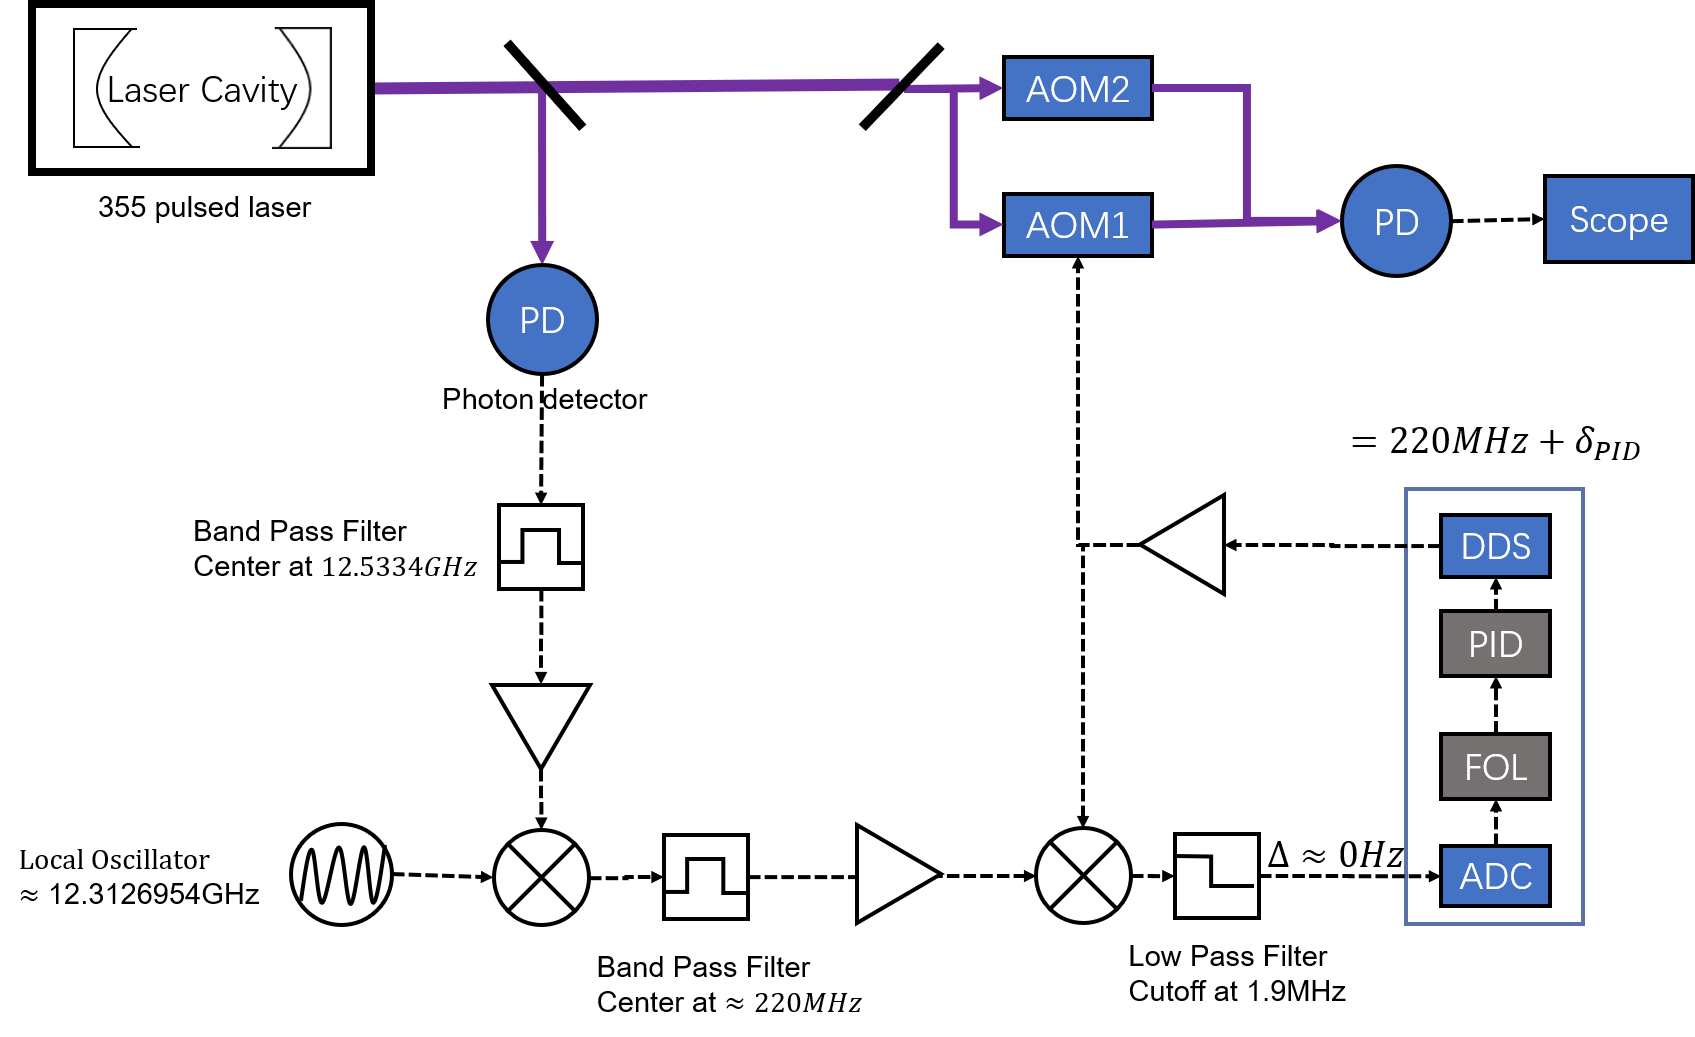
\includegraphics[width=1.0\linewidth]{beat_note_stabilization}
\end{figure}

如图\ref{fig:beat_note_stabilization}所示,为了调整驱动量子比特跃迁的场的频率,来自锁模(脉冲)激光器的光束被分成两条路径,在各自支路上分别受到$\nu_{M1}$和$\nu_{M2}$的频率调制,然后在离子比特上重新交汇。
两条光路尽量等长(不必须严格等长或在光学波长尺度上长期稳定),并需要微调光路长度以使得脉冲能在离子比特处交汇。

图\ref{fig:frequency_comb}显示了由快速光电二极管测量的光束的结果RF光谱,由每个单独光束的激光重复率$\nu_{rep}$分隔,以及经AOM调制后组合光束的$\nu_{rep}\pm |\Delta \nu_M|$分隔的附加拍频边带,其中$|\Delta \nu_M|=|\nu_{M1}-\nu_{M2}|$。
我们通过调整路径$\Delta\nu_M$的相对频移来控制这些额外边带的位置,使之与编码量子信息的能级共振。经调制后用于调控离子的目标边带为$\nu_{sb}$,可以表达为:
\begin{align}
    \nu_{sb}=n\nu_{rep}\pm|\Delta\nu_M|
\end{align}

\begin{figure}
    \centering
    \caption[脉冲激光频率梳]{在频谱分析仪中看到的脉冲激光频率梳\label{fig:frequency_comb}}
    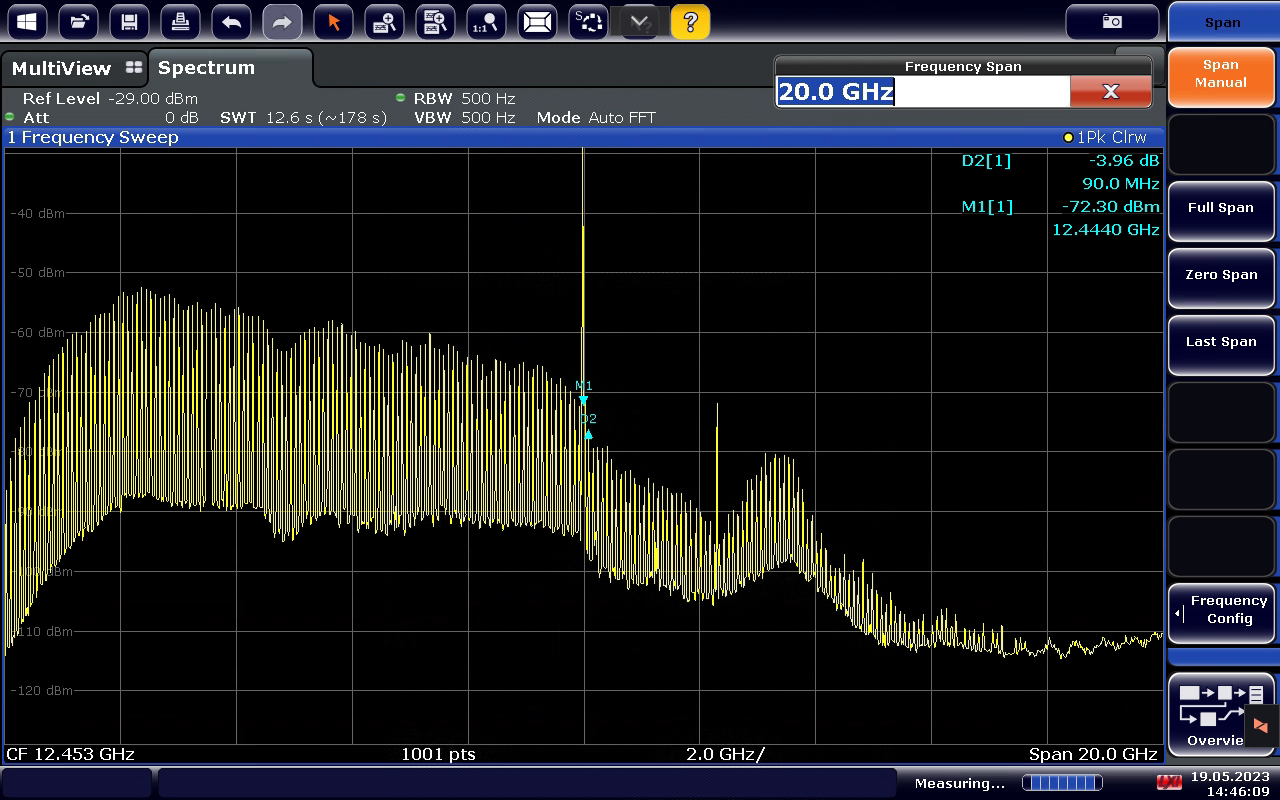
\includegraphics[width=1.0\linewidth]{frequency_comb}
\end{figure}

其中$n$是某个整数,$\nu_{sb}$在频率梳的带宽内。注意采用拉曼跃迁的方式操控时(第\ref{section:raman_transition}节),如图\ref{fig:raman_transition1}所示,激光载波包络相位不需要稳定\cite[]{Peer_Shapiro_Stowe_Shapiro_Ye_2007},尽管也有类似的方式可以完成\cite[]{Koke_Grebing_Frei_Anderson_Assion_Steinmeyer_2010}。

\begin{figure}
    \centering
    \caption[受激拉曼跃迁示意图]{受激拉曼跃迁示意图。$\ket{e}$:上级激发态能级;$\ket{a},\ket{b}$:编码量子信息的高低能级;$\nu_{ab}$:编码量子信息的能级能隙;$\nu_{a}$:$\ket{e}$能级与$\ket{b}$能级的能隙;$\nu_a^L$:$\ket{a}$能级与虚拟能级的能隙;$\nu_b^L$:$\ket{b}$能级与虚拟能级的能隙。\label{fig:raman_transition1}}
    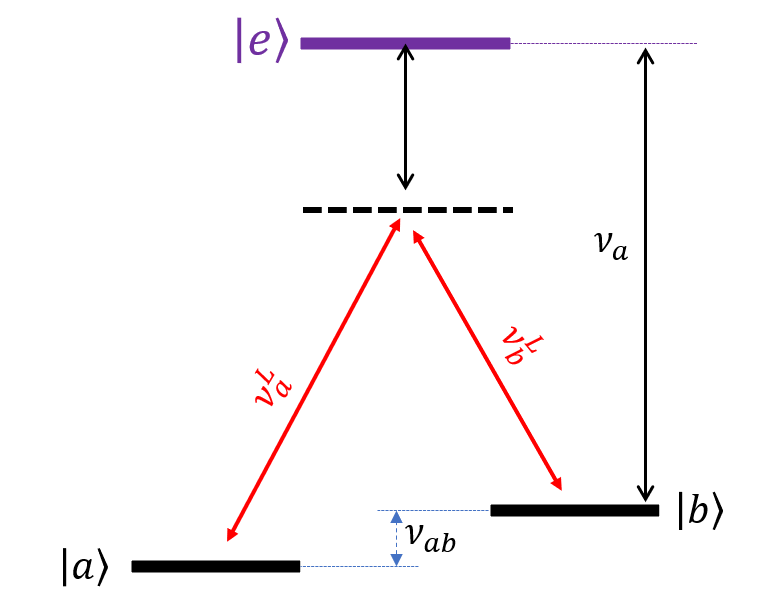
\includegraphics[width=0.6\linewidth]{raman_transition1}
\end{figure}

驱动量子比特需要梳齿之间的光学相干性在量子比特操作的毫秒或更快的时间尺度上保持,这对于锁模(脉冲)激光源来说很容易实现\cite[]{Hayes_Matsukevich_Maunz_Hucul_Quraishi_Olmschenk_Campbell_Mizrahi_Senko_Monroe_2010}。然而,由于激光腔长中的热应变或其它机械应变,激光重复频率会产生漂移[$\nu_{rep}=\nu_{rep}(t)$],导致施加的边带频率$\nu_{sb}$也跟着漂移,进一步地对量子比特驱动也将偏离共振。因此需要一定的措施来稳定用于操控量子比特的边带频率。

可以像密封或光纤激光器的情况一样直接将误差信号反馈给激光腔长,从而稳定重复率,不过当激光腔不容易访问时,这将十分困难。此外,这样的锁的带宽将有限,因为测量激光重复率的采集时间和使用机械换能器调制激光腔长度的延迟可能比激光腔波动的特征时间长。例如,$^{171}Yb$($12.642819 $GHz)电子基态的超精细跃迁在$ \nu_{rep} \sim 80.65$MHz处接近锁模频率激光器的第 157 梳齿。
想要将上述频率稳定在1kHz以内的话,一种经典的方法是测量$\nu_{rep}(t)$使其达到几赫兹的分辨率,而这需要的积分时间将超过1s。这种过于慢的锁定方式并不适合用来锁定频率梳齿的拍频边带。

作为替代,我们选择使用频率梳齿的$n\nu_{rep}(t)$与本地标准参考信号$\nu_{LO}$进行拍频的方式来检测频率的漂动。如图\ref{fig:beat_note_stabilization}所示,我们将锁模(脉冲)激光分出一部分与用FPD进行探测,然后经过一个12.5GHz为中心的带通滤波器并放大后,将其与在12.56GHz附近的本地振荡源拍频。两者拍频之后经过一个合适的低通或带通滤波器就可以获得一个差频信号$|n\nu_{rep}-\nu_{LO}|$(两者的绝对大小不重要,我们总是可以观测到正的差频)。接着将这个差频信号放大并与板卡的DDS输出频率进行拍频和滤波获得一个更小的差频信号,将这个信号送入板卡的AD进行模数转换,随后经过数字滤波器和数字PID的处理对DDS的频率进行调节。整个控制器是采用数字系统实现的,主要涉及模块包括16位AD转换器(Linear Technology, LTC2216)、16位滤波器(第\ref{section:digital_iir}节)、16位PID(第\ref{section:digital_pid}节)、32位DDS(Analog Device, AD9910)。





% 脉冲激光拍频锁定系统原理示意如图\ref{fig:beat_note_stabilization}所示。



\section[脉冲激光拍频锁定系统搭建]{脉冲激光拍频锁定系统搭建}
脉冲激光拍频锁定系统实物
如附录图\ref{fig:beat_note_stabilization_real}所示。
% \begin{figure}
%     \centering
%     \caption[脉冲激光拍频锁定系统图]{脉冲激光拍频锁定系统图\label{fig:beat_note_stabilization_real}}
%     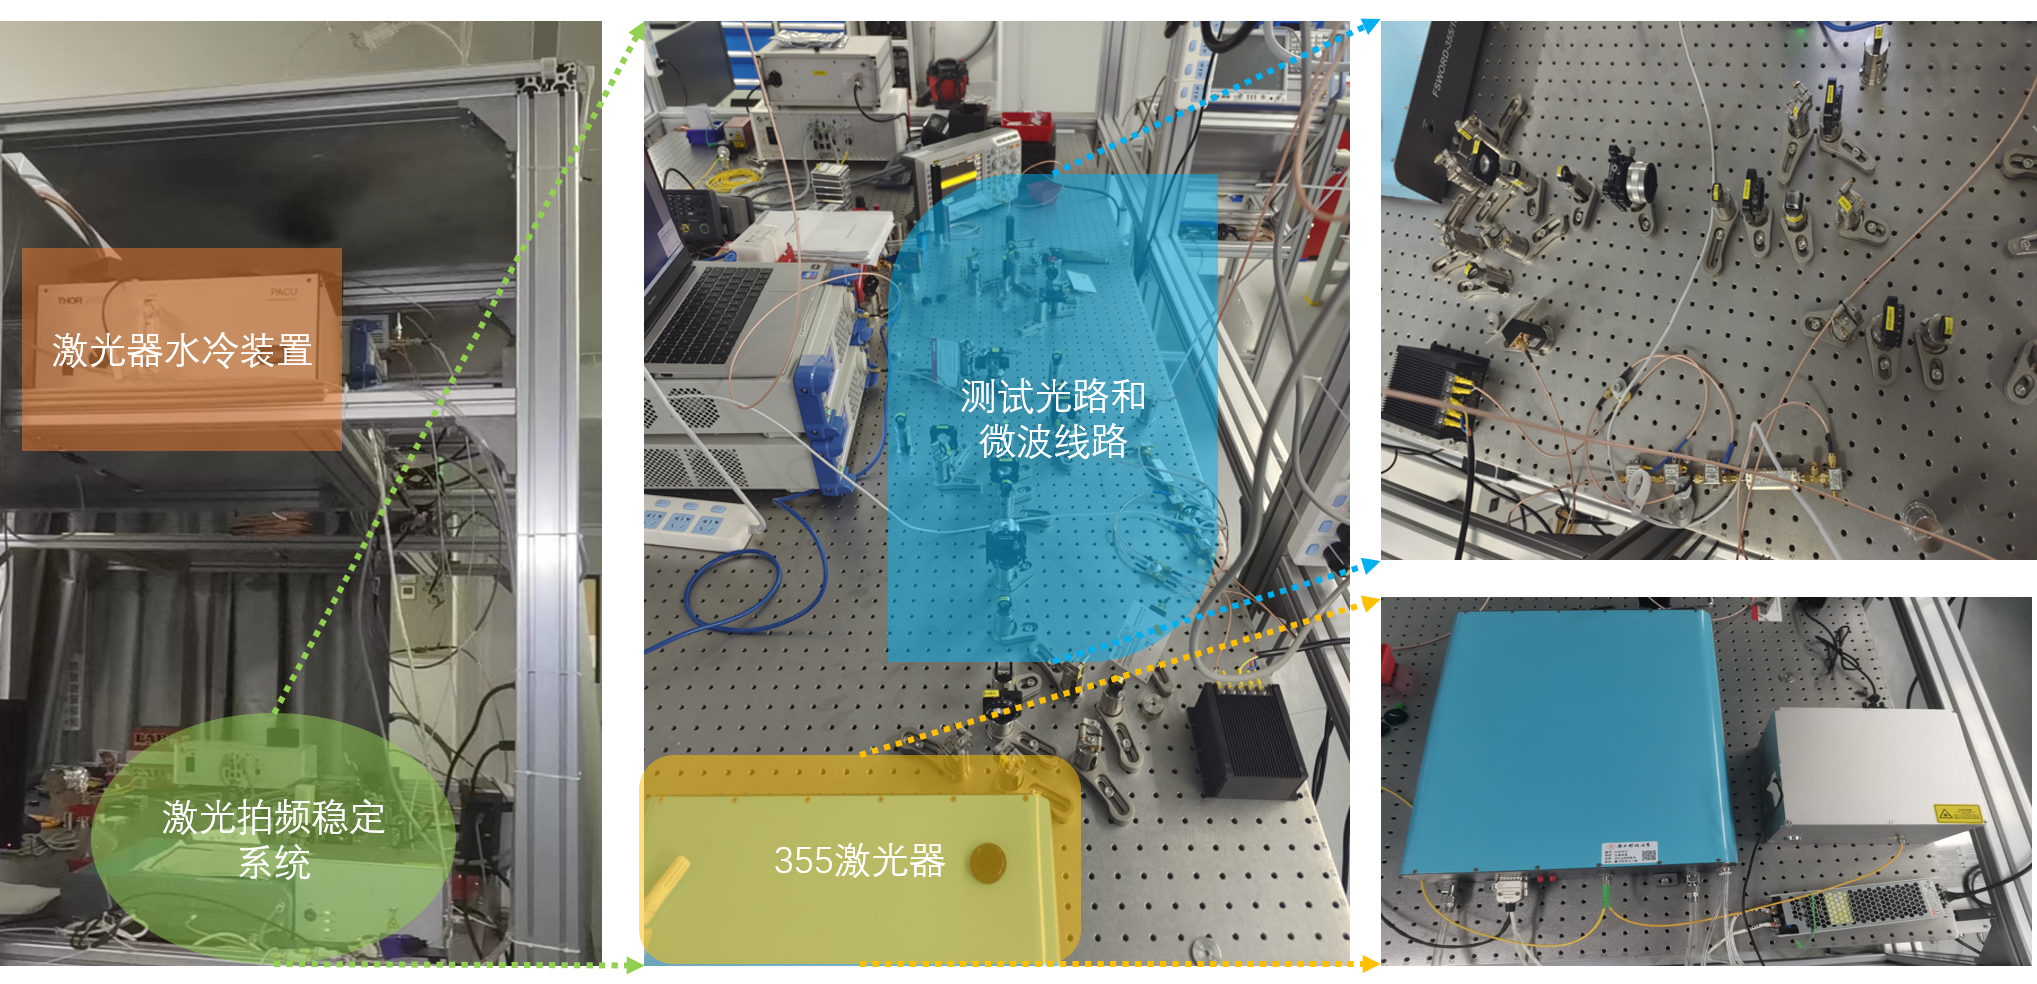
\includegraphics[width=1.0\linewidth]{beat_note_stabilization_real}
% \end{figure}
\newpage
\section[脉冲激光拍频系统锁定结果]{脉冲激光拍频系统锁定结果}
激光拍频锁定的结果如图\ref{fig:beat_note_stabilization_signal}所示,图中展示了在12.39GHz附近的一个稳定的拍频边带。实验中可以利用此类似这样的稳定后的边带与离子进行相互作用,进而实现对离子量子比特的调控。值得一提的是,尽管系统锁定是针对某一级(例如157级)频率梳齿的边带进行锁定的,实际上整个频率梳齿的边带都会一定程度上被稳定下来。不过由于锁模(脉冲)激光重复频率的长期漂动,距离目标锁定边带越远的边带锁定效果越差。
\begin{figure}
    \centering
    \caption[脉冲激光拍频锁定12.39GHz附近稳定边带结果]{脉冲激光拍频锁定12.39GHz附近稳定边带结果\label{fig:beat_note_stabilization_signal}}
    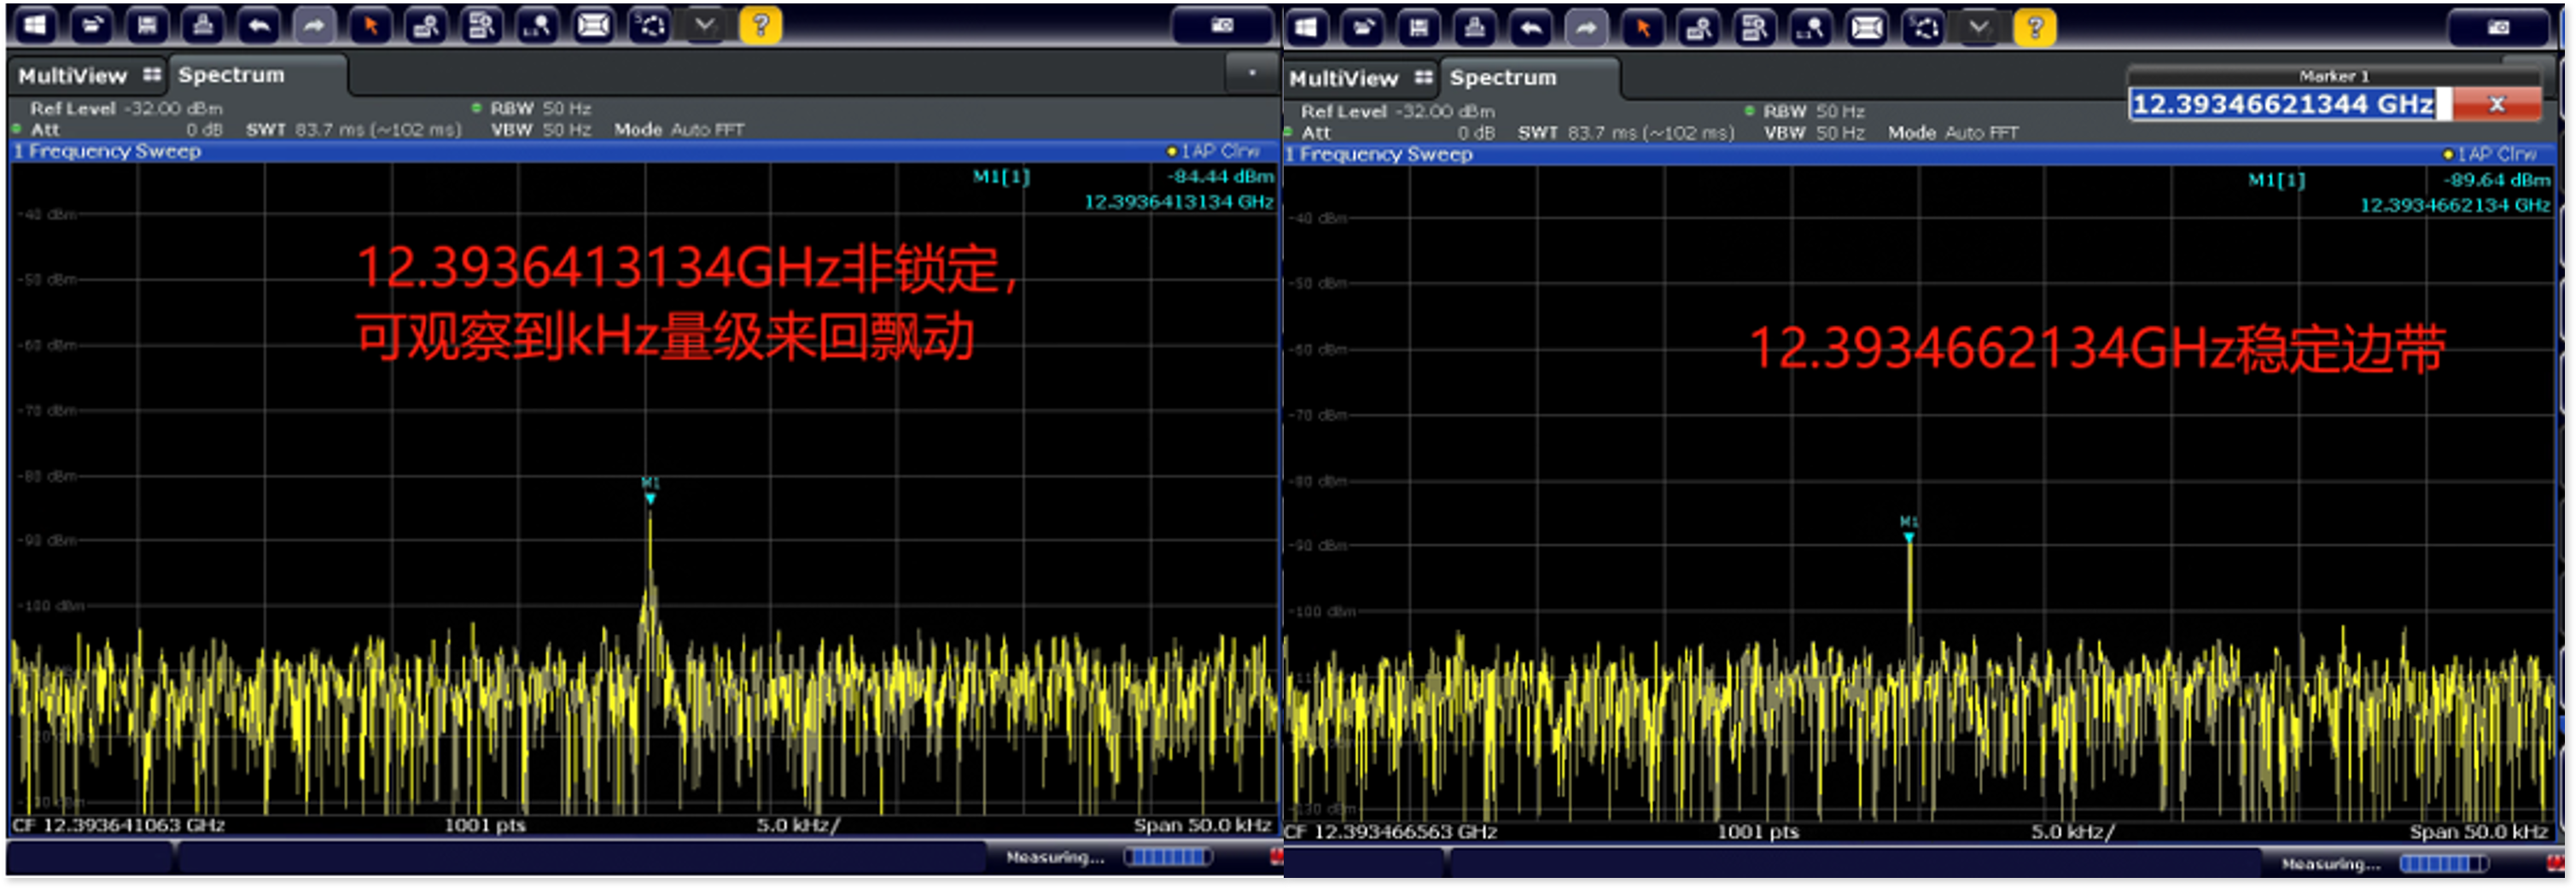
\includegraphics[width=1.0\linewidth]{beat_note_stabilization_signal}
\end{figure}

\subsection[拍频锁定系统的可锁频率幅度]{拍频锁定系统的可锁频率幅度}
由于锁模(脉冲)激光重复频率的长期漂动,数字PID拍频锁定系统需要对其进行补偿来使得频率符合预期值。然而拍频锁定系统并不能应付无限大的频率漂移。\emph{可锁频率幅度}表示了锁频系统对拍频结果的长期漂移的最大可接受范围,超过此范围的长期频率漂动将无法被锁定。下面讨论关于系统的可锁频率幅度相关问题。

该系统结合了大量数字系统,它的控制器和频率输出都由数字系统实现,这及大地提高了系统的稳定性和灵活性。控制器采用了数字PID,调节频率输出采用了DDS。因此理论上只要DDS的输出可以跟得上,应该能锁定接近DDS输出的可调节频率幅度。系统中采用的DDS的频率编码为32bit,频率范围为400MHz。寄存器的数值$R_{DDS}$和实际输出的模拟频率$f_{DDS}$的换算关系为:
\begin{align}
    f_{DDS}=\frac{R_{DDS}}{2^{32}}\times 400\ \textnormal{MHz}
\end{align}

DDS数字对应的\emph{频率步长}为$f_{resolution}=\frac{400\textnormal{MHz}}{2^{32}}\approx0.093\textnormal{Hz}$。然而,DDS芯片中给出的并行频率调制位数是16位,而实际的频率分辨率是32位,这意味着没有办法并行进行全部(0-400MHz)范围内的频率调制。
实际的使用中可以设定一个中心频率$f_{c}$,然后通过16位并行调制字再对这个频率进行微调$\Delta f$。另外,这16位并行调制字可以通过移位$N_{shift}$来对应的32位频率调制字的不同位数,以获得不同的调节范围。每左移一位,并行调制字的权重乘2,最大可移位数为15。也即,16位频率调制字的调制效果$\Delta f$为:
\begin{align}
    \Delta f=f_{resolution}\times n \times 2^{N_{shift}}
\end{align}

其中$n$是16位频率调制字对应的十进制无符号数。最终,DDS的并行调制频率结果为:
\begin{align}
    f_{p}=f_c+f_{resolution}\times n \times 2^{N_{shift}}
\end{align}

需要注意的是在每次的位移后,并行调制的调制频率步长也会增加2倍,也即频率分辨率会相应下降2倍。频率调制字位移数与调制步长的关系如图\ref{fig:beat_note_resolution_shift}所示。

\begin{figure}
    \centering
    \caption[频率调制字位移数vs调制精度
    ]{频率调制字位移数vs调制精度
    \label{fig:beat_note_resolution_shift}}
    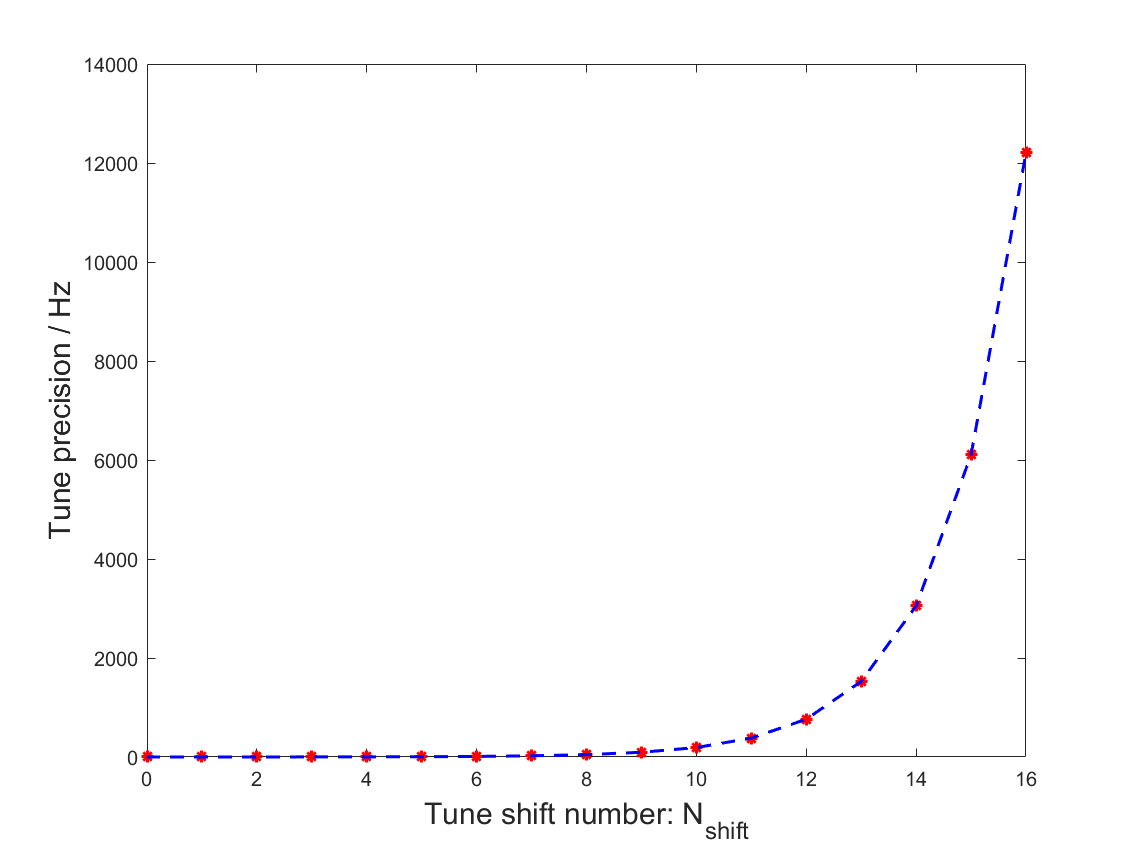
\includegraphics[width=1.0\linewidth]{beat_note_resolution_shift}
\end{figure}


\begin{figure}
    \centering
    \caption[脉冲激光拍频锁定可锁频率幅度测试]{脉冲激光拍频锁定可锁频率幅度测试\label{fig:beat_note_lockable_range_bits}}
    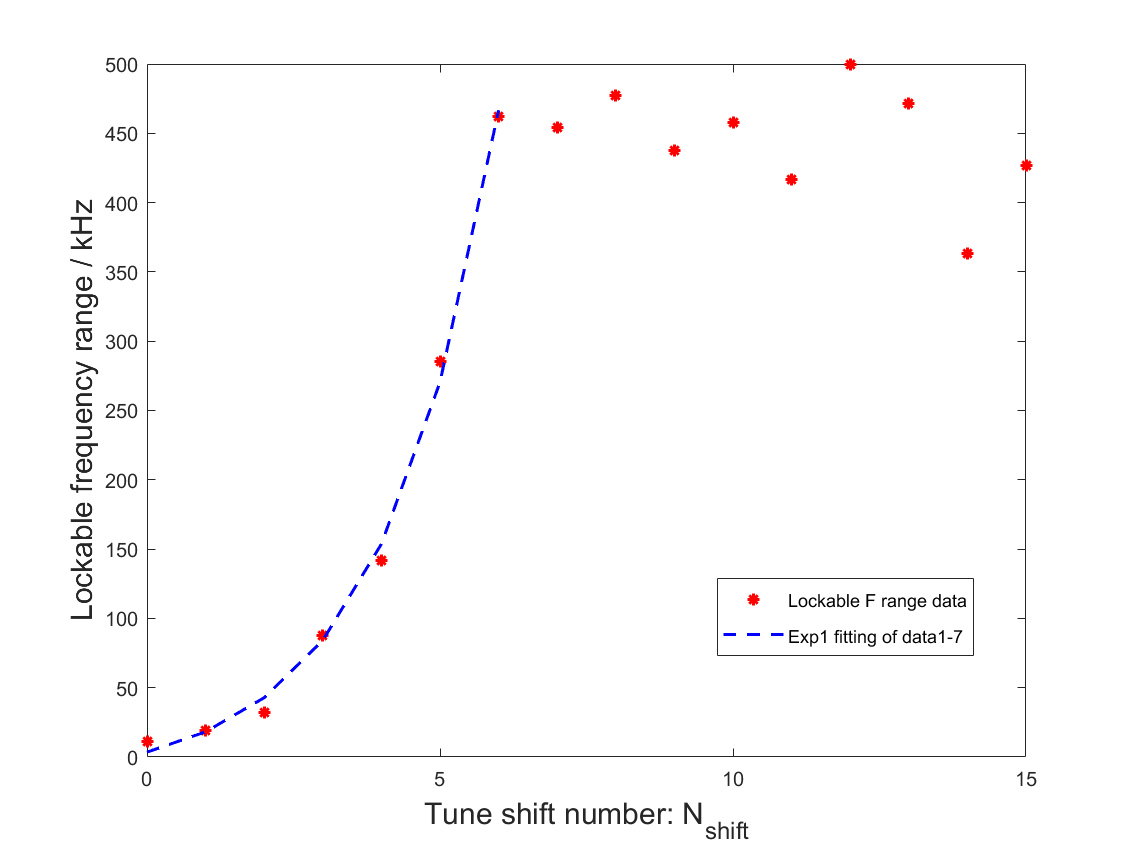
\includegraphics[width=1.0\linewidth]{beat_note_lockable_range_bits}
\end{figure}

通过计算可知,当16位并行调制字移位为0时,可以调节的频率范围仅为约6kHz。在数字PID和DDS的连接一定的情况下,为了测试整个拍频锁定系统的最大可锁频率幅度,可以通过不断移位并行调制字,来测得整个锁频系统最大的可锁频率幅度。测量结果如图\ref{fig:beat_note_lockable_range_bits}所示,理论上在移位到15之前每次移位后测的的可锁频率幅度相对前一种情况应该乘2。从图\ref{fig:beat_note_lockable_range_bits}中可见在移位0-6之间时基本符合这个规律,而到6之后可锁频率幅度便基本保持稳定了。从而可以得出在当前配置下,整个系统的最大可锁频率幅度约为450kHz。这个数值的限制因素主要可能有两个原因:1. 频率调制分辨率过低,导致无法锁定到目标频率上;2. 数字PID带宽影响;3. 系统中存在限制带宽的器件。联系到为了提升调制品质和减少噪声影响,我们的数字系统在PID前添加了一个数字低通滤波器,它的带宽约为450kHz。因此该数字低通滤波器应该是这个结果的主要影响因素。不过由于450kHz的可锁频率范围完全够用了,可以不用再这方面进行进一步优化。如果需要更宽的可锁频率范围,可以通过重新设计该数字低通滤波器的形状和带宽来方便地实现。



